%-----------------------------------------------------------------
%	QUANTUM LIGHT DESCRIPTION
%	!TEX root = ./../main.tex
%-----------------------------------------------------------------
\section{Quantum light description}
\subsection{Classical electrodynamics}
\subsubsection*{Basic equations in the ordinary space}
The basic equations are grouped into two sets. First, the Maxwell equations relate the the electric field $\va{E}(\va{r}, t)$ and the magnetic field $\va{E}(\va{r}, t)$ to the charge density $\rho(\va{r}, t)$ and the current $\va{J}(\va{r}, t)$:
\begin{subequations}
\begin{align}
	\div{E}(\va{r}, t) &= \frac{\rho(\va{r}, t)}{\varepsilon_{0}} \label{eq:max1} \\
	\div{B}(\va{r}, t) &= 0 \label{eq:max2} \\
	\curl{E}(\va{r}, t) &= - \pdv{\va{B}(\va{r}, t)}{t} \label{eq:max3} \\
	\curl{B}(\va{r}, t) &= \frac{1}{c^{2}} \pdv{\va{E}(\va{r}, t)}{t} + \frac{1}{\varepsilon_{0} c^{2}} \va{J}(\va{r}, t) \label{eq:max4}
\end{align}
\end{subequations}
Next, the Newton--Lorentz equation describes the dynamics of each particle $\alpha$ under the influence of electric and magnetic forces exerted by the fields:
\begin{align}
	m_{\alpha} \dv[2]{\va{r}_{a}}{t} = q_{\alpha} \qty[ \va{E}(\va{r}_{\alpha}, t) + \va{v}_{\alpha} \cross \va{B}(\va{r}_{\alpha}, t) ]
\end{align}

The Maxwell's equations implicitly contain the continuity equation ($\pdv*{\rho}{t} + \div{J} \equiv 0$).

The expressions of $\rho(\va{r}, t)$ and $\va{J}(\va{r}, t)$ as a function of the particle variables are
\begin{align}
	\rho(\va{r}, t) &= \sum_{\alpha} q_{\alpha} \delta(\va{r} - \va{r}_{\alpha}(t)) \\
	\va{J}(\va{r}, t) &= \sum_{\alpha} q_{\alpha} \va{v}_{\alpha}(t) \delta(\va{r} - \va{r}_{\alpha}(t))
\end{align}

\subsubsection*{The reciprocal space}
The reciprocal space is the space in which the Fourier transform of a spatial function is represented.
\begin{defi}[Fourier transform]
	A Fourier transform takes us from the ordinary space to the reciprocal space or vice versa:
	\begin{subequations}
	\begin{align}
		\vare{E}(\va{k}, t) &= \frac{1}{(2\pi)^{3/2}} \int \va{E}(\va{r}, t) e^{-i \va{k} \vdot \va{r}} \dd[3]{r} \\
		\va{E}(\va{r}, t) &= \frac{1}{(2\pi)^{3/2}} \int \vare{E}(\va{k}, t) e^{+i \va{k} \vdot \va{r}} \dd[3]{k}
	\end{align}
	\end{subequations}
\end{defi}
% WIP: expand properties?
In this treatment of the space, one frequently uses the following properties of the Fourier transform:
\begin{itemize}
	\item Parseval--Plancherel identity: $\dsp \int F\sast(\va{r}) G(\va{r}) \dd[3]{r} \equiv \int \mc{F}\sast(\va{k}) \mc{G}(\va{k}) \dd[3]{k}$.
	\item Transform of a product (convolution): $\dsp \mc{F}(\va{k})\mc{G}(\va{k}) \leftrightarrow \frac{1}{(2\pi)^{2/3}} \int F(\va{r}\,') G(\va{r} - \va{r}\,') \dd[3]{r'}$.
\end{itemize}

\subsubsection*{Basic equations in the reciprocal space}
Since the $\vnabla$ operator in ordinary space transforms into multiplication by $i \va{k}$ in reciprocal space, Maxwell's equations in reciprocal space become:
\begin{subequations}
\begin{align}
	i\va{k} \vdot \vare{E}(\va{r}, t) &= \frac{\varrho(\va{r}, t)}{\varepsilon_{0}} \\
	i\va{k} \vdot \vare{B}(\va{r}, t) &= 0 \\
	i\va{k} \cross \vare{E}(\va{r}, t) &= - \dot{\vare{B}}(\va{r}, t) \\
	i\va{k} \cross \vare{B}(\va{r}, t) &= \frac{1}{c^{2}} \dot{\vare{E}}(\va{r}, t) + \frac{1}{\varepsilon_{0} c^{2}} \vare{J}(\va{r}, t)
\end{align}
\end{subequations}
The Maxwell's equations implicitly contain the continuity equation ($\dot{\varrho} + i\va{k} \vdot \vare{J} \equiv 0$).

\subsubsection*{Reality condition}
\begin{itemize}
	\item In the ordinary space, a vectorial field is real $\Leftrightarrow \va{E}(\va{r},t) = \va{E}\sast(\va{r},t)$.
	\item In the reciprocal space, a vectorial field is real $\Leftrightarrow \vare{E}(\va{k},t) = \vare{E}\sast(-\va{k},t)$.
\end{itemize}

\subsubsection*{Longitudinal and transverse fields}
Before continuing, it is convenient to distinguish between transverse and longitudinal part of a vector field.
\begin{thm}[Helmholtz theorem]
	For an arbitrary field $\va{V}(\va{r})$, or $\vare{V}(\va{k})$ in the reciprocal space, the Helmholtz theorem states that there is a unique decomposition
	\begin{align}
		\va{V}(\va{r}) = \lng{\va{V}}(\va{r}) + \trn{\va{V}}(\va{r}) \qc \vare{V}(\va{k}) = \lng{\vare{V}}(\va{k}) + \trn{\vare{V}}(\va{k})
	\end{align}
	such that the transverse field is divergence-less
	\begin{align}
		\trn{\div{V}}(\va{r}) = 0 \qc i\va{k} \vdot \trn{\vare{V}}(\va{k}) = 0
	\end{align}
	and the longitudinal field is irrotational
	\begin{align}
		\lng{\curl{V}}(\va{r}) = \va{0} \qc i\va{k} \cross \lng{\vare{V}}(\va{k}) = \va{0}
	\end{align}
\end{thm}

\subsubsection*{Longitudinal electric and magnetic fields}
In the reciprocal space, taking into account the Maxwell's equations and the longitudinal field conditions it's not hard to find an expression for $\lng{\vare{E}}(\va{k})$ and see that the magnetic field is purely transverse:
\begin{align}
	\lng{\vare{E}}(\va{k}) \equiv - \frac{i}{\varepsilon_{0}} \varrho (\va{k}) \frac{\vu{k}}{k} \qc \vare{B}(\va{k}) \equiv \trn{\vare{B}}(\va{k})
\end{align}

Let's now work out the expression for the electric field in the ordinary space:
\begin{flalign*}
	\lng{\va{E}}(\va{r}) & = \mc{F}_{\va{r}}^{-1} \qty{\lng{\vare{E}}(\va{k})} = \mc{F}_{\va{r}}^{-1} \qty{\varrho(\va{k}) \qty(\frac{-i \vu{k}}{\varepsilon_{0} \va{k}})} = \int \rho(\va{r}\,') \frac{1}{4 \pi \varepsilon_{0}} \frac{\va{r} - \va{r}\,'}{\norm{\va{r} - \va{r}\,'}^{3}} \dd[3]{r'}. &
\end{flalign*}
Since charge density is defined as $\rho(\va{r}) \equiv \sum_{\alpha} q_{\alpha} \delta(\va{r} - \va{r}_{\alpha})$, we find the expression of the Coulomb field:
\begin{align}
	\lng{\va{E}}(\va{r}) = \frac{1}{4 \pi \varepsilon_{0}} \sum_{\alpha} q_{\alpha} \frac{\va{r} - \va{r}_{\alpha}}{\norm{\va{r} - \va{r}_{\alpha}}^{3}}
\end{align}
Therefore this is not important to the evolution of the electric field itself; it's just related to the particles.

\subsubsection*{Transverse electric and magnetic fields}
In the reciprocal space, taking into account the Maxwell's equations and the transverse field conditions it's not hard to find expressions for the temporal evolution of $\vare{B}$ and $\trn{\vare{E}}$:
\begin{align}
	\trn{\dot{\vare{E}}} = i c^{2} \va{k} \cross \vare{B} - \frac{1}{\varepsilon_{0}} \trn{\vare{J}} \qc \dot{\vare{B}} = - i \va{k} \cross \trn{\vare{E}}
\end{align}

Apart from that, we can also derive the continuity equation in the reciprocal space:
\begin{flalign*}
	\frac{\lng{\dot{\vare{E}}}}{c^{2}} + \frac{1}{\varepsilon_{0} c^{2}} \lng{\vare{J}} &= 0 \Rightarrow \va{k} \vdot \lng{\dot{\vare{E}}} + \frac{1}{\varepsilon_{0}} \va{k} \vdot (\lng{\vare{J}} + \trn{\vare{J}}) = 0 \Rightarrow \dot{\varrho} + i\va{k} \vdot \vare{J} \equiv 0. &
\end{flalign*}

\subsubsection*{Normal variables}
Let's assume for a moment (for the sake of simplification) that $\trn{\vare{J}} = \va{0}$. Multiplying $\va{k}$ vectorially with the expression we found for the temporal evolution of the magnetic field (and keeping in mind that $\va{A} \cross \va{B} \cross \va{C} = \va{A} (\va{B} \vdot \va{C}) - \va{C} (\va{A} \vdot \va{B})$), we get
\begin{flalign*}
	\va{k} \cross (\dot{\vare{B}} &= - i \va{k} \cross \trn{\vare{E}}) \Rightarrow \va{k} \cross \dot{\vare{B}} = i k^{2} \trn{\vare{E}} &
\end{flalign*}
Mixing this result with the expression for the temporal evolution of the transverse electric field, we get
\begin{align*}
	\pdv{t} \qty( \trn{\vare{E}} \pm c \vu{k} \cross \vare{B}) = \pm i c k \qty( \trn{\vare{E}} \pm c \vu{k} \cross \vare{B})
\end{align*}

One is then led to define, even if $\trn{\vare{J}} \neq \va{0}$, two new variables $\va{\alpha}(\va{k}, t)$ and $\va{\beta}(\va{k}, t)$.

\begin{defi}[Normal variables]
	\begin{subequations}
	\begin{align}
		\va{\alpha}(\va{k}, t) &\equiv - \frac{i}{2 N(k)} \qty[ \trn{\vare{E}} - c \va{k} \cross \vare{B} ] \\
		\va{\beta}(\va{k}, t) &\equiv - \frac{i}{2 N(k)} \qty[ \trn{\vare{E}} + c \va{k} \cross \vare{B} ]
	\end{align}
	\end{subequations}
	where $N(k)$ is a normalisation factor which will be chosen later. The real character of $\trn{\vare{E}}$ and $\vare{B}$ requires that $\va{\beta}(\va{k}, t) \equiv \va{\alpha}\sast(-\va{k}, t) = \va{\alpha}_{-}\sast$. Therefore we can forget about $\va{\beta}$ and write everything in terms of $\va{\alpha}$.
\end{defi}

Since $\va{\alpha}$ is (like $\trn{\vare{E}}$ and $\vare{B}$) a transverse vector field, one can, for each value of $\va{k}$, expand $\va{\alpha}(\va{k},t)$ on two unit vectors $\vu{\epsilon}$ and $\vu{\epsilon}'$, normal to each other and both located in the plane perpendicular to propagation vector. Therefore, we can always write the normal vector as
\begin{align}
	\va{\alpha}(\va{k}, t) \equiv \sum_{\epsilon} \alpha_{\epsilon}(\va{k}, t) \vu{\epsilon}
\end{align}
where $\vu{\epsilon}$ is the transverse polarisation vector, and $\alpha_{\epsilon}(\va{k}, t)$ is the projection of $\va{\alpha}$ into $\vu{\epsilon}$.

Let's rewrite the transverse expression for the electric and the magnetic fields in terms of the normal variables:
\begin{subequations}
\begin{align}
	\trn{\vare{E}} &= i N(k) \qty[ \va{\alpha} - \va{\alpha}_{-}\sast ] \\
	\vare{B} &= \frac{i N(k)}{c} \qty[ \vu{k} \cross \va{\alpha} + \vu{k} \cross \va{\alpha}_{-}\sast ]
\end{align}
\end{subequations}

\subsubsection*{Evolution of the normal variable}
\begin{align}
	\dot{\va{\alpha}} + i \omega \va{\alpha} = \dfrac{i}{2 \varepsilon_{0} N(k)} \trn{\vare{J}}
\end{align}
This can be interpreted as an harmonic oscillator (with $\omega \equiv ck$). Therefore, to completely describe a system at $t_{0}$, we only need to know $\qty{\va{\alpha}(\va{k}, t_{0}), \va{r}_{\alpha}(t_{0}), \va{v}_{\alpha}(t_{0})}$.

\subsubsection*{Energy in terms of the normal variable}
The energy can be defined as the sum of the kinetic and potential energies:
\begin{align}
	H = \sum_{\alpha} \frac{1}{2} m_{\alpha} v^{2}_{\alpha} (t) + \frac{\varepsilon_{0}}{2} \int \qty(E^{2} + c^2 B^{2}) \dd[3]{r}
\end{align}
Let's simplify the terms of the potential energy:
\begin{flalign*}
	\frac{\varepsilon_{0}}{2} \int E^{2} \dd[3]{r} &= \frac{\varepsilon_{0}}{2} \int \qty(\lng{\va{E}} + \trn{\va{E}})^{2} \dd[3]{r} = \frac{\varepsilon_{0}}{2} \int \qty(\lng{E}^{2} + \trn{E}^2 + \cancel{2 \lng{\va{E}} \vdot \trn{\va{E}}}) \dd[3]{r} & \\
	&\Rightarrow \frac{\varepsilon_{0}}{2} \int \qty(E^{2} + c^2 B^{2}) \dd[3]{r} = \underbrace{\frac{\varepsilon_{0}}{2} \int \lng{E}^{2} \dd[3]{r}}_{\lng{H}, \text{ longitudinal}} + \underbrace{\frac{\varepsilon_{0}}{2} \int \qty(\trn{E}^2 + c^{2} B^{2}) \dd[3]{r}}_{\trn{H}, \text{ transverse}} \\
\end{flalign*}
The Coulomb and transverse parts of the potential energy can be simplified further:
\begin{flalign*}
	\lng{H} &= \frac{\varepsilon_{0}}{2} \int \lng{E}^{2} \dd[3]{r} \overset{\text{P. Id.}}{=} \frac{\varepsilon_{0}}{2} \int \lng{\vare{E}}\sast \lng{\vare{E}} \dd[3]{k} = \frac{1}{2 \varepsilon_{0}} \int \varrho\sast(\va{k}) \frac{\varrho(\va{k})}{k^{2}} \dd[3]{k} \qc \varrho(\va{k}) = \sum_{\alpha} \frac{q_{\alpha}}{(2\pi)^{3/2}} e^{-i \va{k} \vdot \va{r}_{\alpha}} & \\
	&\Rightarrow \lng{H} = \sum_{\alpha \neq \beta} \frac{q_{\alpha} q_{\beta}}{2 \varepsilon_{0} (2 \pi)^{3}} \int \frac{e^{-i \va{k} \vdot (\va{r}_{\alpha} - \va{r}_{\beta})}}{k^{2}} \dd[3]{k} = \frac{1}{8 \pi \varepsilon_{0}} \sum_{\alpha \neq \beta} \frac{q_{\alpha} q_{\beta}}{\norm{\va{r}_{\alpha} - \va{r}_{\beta}}} \equiv H_{C} \\
	\trn{H} &= \frac{\varepsilon_{0}}{2} \int \qty(\trn{E}^2 + c^{2} B^{2}) \dd[3]{r} = \frac{\varepsilon_{0}}{2} \int \qty(\trn{\va{E}}\sast \vdot \trn{\va{E}} + c^{2} \va{B}\sast \vdot \va{B}) \dd[3]{r} \\
	&\overset{\text{P. Id.}}{=} \frac{\varepsilon_{0}}{2} \int \qty(\trn{\vare{E}}\sast \vdot \trn{\vare{E}} + c^{2} \vare{B}\sast \vdot \vare{B}) \dd[3]{r} = \varepsilon_{0} \int N^{2} \qty( \va{\alpha}\sast \vdot \va{\alpha} + \va{\alpha}_{-} \vdot \va{\alpha}_{-}\sast ) \dd[3]{k} \\
	&= \varepsilon_{0} \int N^{2} \qty( \va{\alpha}\sast \vdot \va{\alpha} + \va{\alpha} \vdot \va{\alpha}\sast ) \dd[3]{k} = \varepsilon_{0} \int \frac{\hbar \omega}{2} \qty( \va{\alpha}\sast \vdot \va{\alpha} + \va{\alpha} \vdot \va{\alpha}\sast ) \dd[3]{k}
\end{flalign*}
where we have defined the normalisation factor as $N(k) \equiv \sqrt{\dfrac{\hbar \omega}{2}}$.

Therefore, we have seen that the energy can be expressed in a more compact way:
\begin{subequations}
\begin{align}
	H = \sum_{\alpha} \frac{1}{2} m_{\alpha} v^{2}_{\alpha} (t) + H_{C} + \trn{H}
\end{align}
where the Coulomb (or longitudinal) and transverse potentials can be respectively written as
\begin{align}
	H_{C} = \frac{1}{8 \pi \varepsilon_{0}} \sum_{\alpha \neq \beta} \frac{q_{\alpha} q_{\beta}}{\norm{\va{r}_{\alpha} - \va{r}_{\beta}}} \qc \trn{H} = \varepsilon_{0} \int \frac{\hbar \omega}{2} \qty( \va{\alpha}\sast \vdot \va{\alpha} + \va{\alpha} \vdot \va{\alpha}\sast ) \dd[3]{k}
\end{align}
\end{subequations}
From the expression of $\trn{H}$, one can think of the electromagnetic field can be as the sum of harmonic oscillators of frequency $\omega$ being associated with each pair of vectors $\va{k}$, $\vu{\epsilon}$. Such a pair defines a mode of the transverse field.

\subsubsection*{Linear momentum in terms of the normal variable}
The total linear momentum is the sum of the particle mechanical momenta $m_{\alpha} \va{v}_{\alpha}$ and the field momentum:
\begin{subequations}
\begin{align}
	\va{P} = \sum_{\alpha} m_{\alpha} \va{v}_{\alpha} + \varepsilon_{0} \int \qty(\va{E} \cross \va{B}) \dd[3]{r}
\end{align}

Having in mind that $\va{E} = \lng{\va{E}} + \trn{\va{E}}$, doing a calculation similar to that for $\trn{H}$, we can find an expression for the the transverse part of the linear momentum:
\begin{align}
	\trn{\va{P}} = \varepsilon_{0} \int \qty(\trn{\va{E}} \cross \va{B}) \dd[3]{r} = \int \frac{\hbar \va{k}}{2} \qty(\va{\alpha}\sast \vdot \va{\alpha} + \va{\alpha} \vdot \va{\alpha}\sast) \dd[3]{k}
\end{align}
\end{subequations}

\subsubsection*{Electric and magnetic fields in ordinary space}
To find the expression for the electric field in the ordinary space we just need to apply the inverse Fourier transform:
\begin{flalign*}
		\trn{\va{E}}(\va{r}, t) &\equiv \frac{1}{(2\pi)^{3/2}} \int \trn{\vare{E}}(\va{k}, t) e^{i \va{k} \vdot \va{r}} \dd[3]{k} = \int \sqrt{\frac{\hbar \omega}{2 \varepsilon_{0}}} \frac{i}{(2\pi)^{3/2}} \qty(\va{\alpha} - \va{\alpha}_{-}\sast) e^{i \va{k} \vdot \va{r}} \dd[3]{k} & \\
		&= \int \sqrt{\frac{\hbar \omega}{2 \varepsilon_{0}}} \frac{i}{(2\pi)^{3/2}} \sum_{\epsilon} \qty(\alpha_{\epsilon} \vu{\epsilon} \, e^{i \va{k} \vdot \va{r}} - \alpha_{\epsilon -}\sast \vu{\epsilon} \, e^{i \va{k} \vdot \va{r}}) \dd[3]{k} \\
		&= \int \sqrt{\frac{\hbar \omega}{2 \varepsilon_{0}}} \frac{i}{(2\pi)^{3/2}} \sum_{\epsilon} \qty(\alpha_{\epsilon} \vu{\epsilon} \, e^{i \va{k} \vdot \va{r}} - \alpha_{\epsilon}\sast \vu{\epsilon} \, e^{-i \va{k} \vdot \va{r}}) \dd[3]{k} \\
\end{flalign*}
Therefore, the transverse electric field in the ordinary space is
\begin{subequations}
\begin{align}
	\trn{\va{E}}(\va{r}, t) = i \int \sum_{\epsilon} \mc{E}_{\omega} \qty(\alpha_{\epsilon}(\va{k}, t) \vu{\epsilon} \, e^{i \va{k} \vdot \va{r}} - \alpha_{\epsilon}\sast(\va{k}, t) \vu{\epsilon} \, e^{-i \va{k} \vdot \va{r}}) \dd[3]{k}
\end{align}
where $\mc{E}_{\omega} \equiv \dfrac{1}{(2\pi)^{3/2}}\sqrt{\dfrac{\hbar \omega}{2 \varepsilon_{0}}}$ is the amplitude of the reciprocal electric field.

For the magnetic field in the ordinary space we get a similar expression:
\begin{align}
	\trn{\va{B}}(\va{r}, t) = i \int \sum_{\epsilon} \mc{B}_{\omega} \qty(\alpha_{\epsilon}(\va{k}, t) \vu{k} \cross \vu{\epsilon} \, e^{i \va{k} \vdot \va{r}} - \alpha_{\epsilon}\sast(\va{k}, t) \vu{k} \cross \vu{\epsilon} \, e^{-i \va{k} \vdot \va{r}}) \dd[3]{k}
\end{align}
\end{subequations}
where $\mc{B}_{\omega} \equiv \dfrac{\mc{E}_{\omega}}{c}$ is the amplitude of the reciprocal magnetic field.

\subsubsection*{Vector potential}
We can express the electric and the magnetic fields in term of the vector potential:
\begin{align}
	\va{E}(\va{r},t) = - \dv{\va{A}(\va{r},t)}{t} - \grad{U}(\va{r},t) \qc \va{B}(\va{r},t) = \curl{A}(\va{r},t)
\end{align}

Choosing the Coulomb gauge ($\div{A} \equiv 0$), we see that the vector potential is purely transverse. Therefore, it's quite obvious that
\begin{align*}
	\trn{\va{E}} = - \dv{\trn{\va{A}}}{t} \qc \lng{\va{E}} = - \grad{U}
\end{align*}

We can also find the expressions for the the electric and magnetic fields in the reciprocal space:
\begin{align*}
	\trn{\vare{E}} = - \trn{\dot{\vare{A}}} \qc \vare{B} = i \va{k} \cross \trn{\vare{A}}
\end{align*}
Therefore, the transverse vector potential can be written as
\begin{align}
	\trn{\vare{A}} \equiv \sqrt{\frac{\hbar}{2 \varepsilon_{0} \omega}} \qty(\va{\alpha} + \va{\alpha}_{-}\sast)
\end{align}

This expression makes possible to find the normal vector, $\va{\alpha}$, as a function of $\trn{\vare{A}}$ and $\trn{\vare{E}}$:
\begin{align}
	\va{\alpha}(\va{k},t) = \frac{1}{2 N(k)} \qty[\omega \trn{\vare{A}}(\va{k},t) - i \trn{\vare{E}}(\va{k},t)]
\end{align}

\subsubsection*{Periodic boundary conditions}
A useful mathematical trick to quantise the fields is to define a cube of lateral size $L$ and impose periodic boundary conditions:
\begin{align*}
	\trn{\va{E}}(\va{r} + \vu{x} L) = \trn{\va{E}}(\va{r} + \vu{y} L) = \trn{\va{E}}(\va{r} + \vu{z} L)
\end{align*}
In this way $\va{k}$ becomes discrete: $\va{k}_{x,y,z} = \dfrac{2\pi}{L} \vu{k}_{x,y,z}$.

Therefore, we can rewrite everything in terms of the discrete $\va{k}_{r}$:
\begin{align}\label{eq:disc-cont}
	\sum_{\va{k}_{j}} \qty(\frac{2\pi}{L})^{3} f(\va{k}_{j}, \vu{\epsilon}_{j}) \underset{L \to \infty}{\longrightarrow} \int f(\va{k}, \vu{\epsilon}) \dd[3]{k}
\end{align}
The notation we will use is $\alpha_{\va{k}_{j},\vu{\epsilon}_{j}} \mapsto \alpha_{j}$, therefore all the sums are just over $j$:
\begin{subequations}
\begin{align}
	\trn{\va{A}} &= \sum_{j} \mc{A}_{\omega_{j}} \qty{\alpha_{j} \vu{\epsilon}_{j} e^{i \va{k}_{j} \vdot \va{r}} + \cc} \qc \mc{A}_{\omega_{j}} = \frac{\mc{E}_{\omega_{j}}}{\omega_{j}} \\
	\trn{\va{E}} &= i \sum_{j} \mc{E}_{\omega_{j}} \qty{\alpha_{j} \vu{\epsilon}_{j} e^{i \va{k}_{j} \vdot \va{r}} - \cc} \qc \mc{E}_{\omega_{j}} = \sqrt{\frac{\hbar \omega_{j}}{2 \varepsilon_{0} L^{3}}} \\
	\trn{\va{B}} &= i \sum_{j} \mc{B}_{\omega_{j}} \qty{\alpha_{j} \va{k}_{j} \cross \vu{\epsilon}_{j} e^{i \va{k}_{j} \vdot \va{r}} - \cc} \qc \mc{B}_{\omega_{j}} = \frac{\mc{E}_{\omega_{j}}}{c} \\
	\trn{H} &= \sum_{j} \frac{1}{2} \hbar \omega_{j} \qty{\alpha_{j}\sast \alpha_{j} + \cc} \\
	\trn{\va{P}} &= \sum_{j} \frac{1}{2} \hbar \va{k}_{j} \qty{\alpha_{j}\sast \alpha_{j} + \cc}
\end{align}
\end{subequations}

%-----------------------------------------------------------------
\subsection{Quantisation of the electromagnetic field}
\begin{subequations}
\begin{align}
	\trn{\va{E}} &= i \sum_{j} \mc{E}_{\omega_{j}} \qty{\hat{a}_{j} \vu{\epsilon}_{j} e^{i \va{k}_{j} \vdot \va{r}} - \Hc} \\
	\trn{\va{B}} &= i \sum_{j} \mc{B}_{\omega_{j}} \qty{\hat{a}_{j} \va{k}_{j} \cross \vu{\epsilon}_{j} e^{i \va{k}_{j} \vdot \va{r}} - \Hc} \\
	\trn{H} &= \sum_{j} \hbar \omega_{j} \qty(\hat{a}_{j}\sdag \hat{a}_{j} + \frac{1}{2} ) \\
	\trn{\va{P}} &= \sum_{j} \hbar \va{k}_{j} \qty(\hat{a}_{j}\sdag \hat{a}_{j})
\end{align}
\end{subequations}
It's important to note that $\trn{\va{E}}$ and $\trn{\va{B}}$ are local operators, while $\trn{H}$ and $\trn{\va{P}}$ are global operators.

%-----------------------------------------------------------------
\subsection{Fock states}
\begin{defi}[Fock state, $\ket{n_{j}}$]
	For one mode of the electromagnetic field, we can define the state $\ket{n_{j}}$ for any non-negative $n_{j}$ such that
	\begin{subequations}
	\begin{align}
		\hat{a}_{j} \ket{n_{j}} &= \sqrt{n_{j}}\ket{n_{j} - 1} \\
		\hat{a}_{j}\sdag \ket{n_{j}} &= \sqrt{n_{j} + 1}\ket{n_{j} + 1} \\
		\hat{N}_{j} \ket{n_{j}} &= \hat{a}_{j}\sdag \hat{a}_{j} \ket{n_{j}} = n_{j} \ket{n_{j}}
	\end{align}
	\end{subequations}
	In quantum optics, $\ket{n}$ can be interpreted as a system of $n$ photons.
\end{defi}

\subsubsection*{Properties of the Fock states}
\begin{enumerate}[i)]
	\item They are orthogonal: $\braket{n_{j}}{m_{j}} \equiv \prod_{j} \delta_{n_{j},m_{j}}$.
	\item They form a complete base: $\sum_{j} \dyad{n_{j}}{n_{j}} \equiv \bbid$.
\end{enumerate}

To each mode of the electromagnetic field, it corresponds one Fock state. Since the electromagnetic field has infinite modes,
\begin{align*}
	\ket{n_{1}} \otimes \ket{n_{2}} \otimes \cdots \otimes \ket{n_{j}} \otimes \cdots \equiv \ket{n_{1}, n_{2}, \cdots, n_{j}, \cdots}
\end{align*}

It's easy to see that the Fock states are eigenstates of the transverse part of the energy and the momentum:
\begin{subequations}
\begin{align}
	\trn{H} \ket{n_{1}, n_{2}, \cdots, n_{j}, \cdots} &= \sum_{j} \hbar \omega_{j} \qty(n_{j} + \frac{1}{2} ) \ket{n_{1}, n_{2}, \cdots, n_{j}, \cdots} \\
	\trn{\va{P}} \ket{n_{1}, n_{2}, \cdots, n_{j}, \cdots} &= \sum_{j} \hbar \va{k}_{j} n_{j} \ket{n_{1}, n_{2}, \cdots, n_{j}, \cdots}
\end{align}
\end{subequations}
Therefore, $\trn{H}$ and $\trn{\va{P}}$ give us the corpuscular nature of the system.

\begin{align*}
	\trn{\va{E}} &\ket{n_{1}, n_{2}, \cdots, n_{j}, \cdots} = i \sum_{j} \mc{E}_{\omega_{j}} \qty{\hat{a}_{j} \vu{\epsilon}_{j} e^{i \va{k}_{j} \vdot \va{r}} - \Hc} \ket{n_{1}, n_{2}, \cdots, n_{j}, \cdots} \\
	% &= f(\hat{a}) \ket{n_{1}, n_{2}, \cdots, n_{j}, \cdots} \\
	& \Rightarrow \ev{{\va{E}}}{n_{1}, n_{2}, \cdots, n_{j}, \cdots} \equiv 0
\end{align*}
Since $\trn{\va{E}}$ is a linear function of $\hat{a}_{j}$, this result is obvious. This means that the electric field gives no information about the wave nature of the system.

%-----------------------------------------------------------------
\subsection{Vacuum states}
\begin{defi}[Vacuum state, $\ket{0}$]
	The vacuum state is the quantum state with the lowest possible energy (zero-point energy):
	\begin{align}
		\trn{H} \ket{0} = \sum_{j} \frac{1}{2} \hbar \omega_{j} \ket{0} \Rightarrow E_{0} = \sum_{j} \frac{1}{2} \hbar \omega_{j} = \infty
	\end{align}
\end{defi}

\subsubsection*{Manifestations of the vacuum}
\begin{itemize}
	\item Since $\sum$ has less possible modes than $\int$, therefore $\grad{E} \neq \va{0}$, there's a force between the plates, called \emph{Casimir force}.
	\begin{figure}[H]
		\centering
		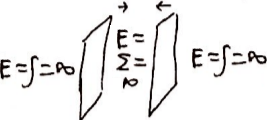
\includegraphics[width=0.32\textwidth]{./images/4-casimir}
		\caption{Casimir force between two parallel plates}
		\label{fig:casimir}
	\end{figure}
	\item The \emph{Lamb shift} is responsible of the breaking of the degeneracy between states $2 \, ^{2}s_{1/2}$ and $2 \, ^{2}p_{1/2}$ of hydrogen.
\end{itemize}

\subsubsection*{Spontaneous emission}
\begin{flalign*}
	\trn{E}^{2} &= -\sum_{j} \frac{\hbar \omega_{j}}{2 \varepsilon_{0} L^{3}} \qty(\cancel{\hat{a}_{j} \hat{a}_{j} e^{2i \va{k}_{j}\vdot\va{r}}} - \hat{a}_{j} \hat{a}_{j}\sdag - \cancel{\hat{a}_{j}\sdag \hat{a}_{j}} + \cancel{\hat{a}_{j}\sdag \hat{a}_{j}\sdag e^{-2i \va{k}_{j}\vdot\va{r}}} ) \Rightarrow \ev{\trn{E}^{2}}_{\ket{0}} = \sum_{j} \frac{\hbar \omega_{j}}{2 \varepsilon_{0} L^{3}} &
\end{flalign*}
But to recover the physical meaning, we need to do the limit when $L \to \infty$:
\begin{flalign*}
	\sum_{j} \frac{\hbar \omega_{j}}{2 \varepsilon_{0} L^{3}} &= \sum_{k_{j}} \sum_{\epsilon_{j}} \frac{\hbar c k_{j}}{2 \varepsilon_{0} L^{3}} \frac{(2\pi)^{3}}{(2\pi)^{3}} = \sum_{k_{j}} \frac{\hbar c k_{j}}{\varepsilon_{0} (2\pi)^{3}} \qty(\frac{2\pi}{L})^{3} & \\
	&\Rightarrow \int \frac{\hbar c k}{\varepsilon_{0} (2\pi)^{3}} \dd[3]{k} = \frac{\hbar c}{\varepsilon_{0} (2\pi)^{3}} \int k (k^{2} \dd{k} \dd{\Omega}) = \frac{\hbar c 4\pi}{\varepsilon_{0} (2\pi)^{3}} \int k^{3} \dd{k}
\end{flalign*}
Therefore,
\begin{align}
	(\Delta \trn{E}^{2})_{\ket{0}} = \ev{\trn{E}^{2}}{0} = \frac{\hbar c}{2 \varepsilon_{0} \pi^{2}} \int k^{3} \dd{k}
\end{align}
These fluctuations in the electric field are responsible of the spontaneous emission.

%-----------------------------------------------------------------
\subsection[Coherent states]{Coherent/quasi-classical states}
\begin{defi}[Coherent state, $\ket{\alpha}$]
	The coherent state is the eigenstate of the annihilation operator:
	\begin{subequations}
	\begin{align}
		\hat{a} \ket{\alpha} &= \alpha \ket{\alpha} \\
		\bra{\alpha} \hat{a}\sdag &= \alpha\sast \bra{\alpha} \\
		\comm*{\hat{a}}{\hat{a}\sdag} &\equiv \hat{\bbid}
	\end{align}
	\end{subequations}
\end{defi}
Coherent states are also called quasi-classical states because the expected values of the global and local operators correspond to the values of the classical fields:
\begin{align*}
	\left.
	\begin{aligned}
		\ev{\va{A}}{\alpha_{j}} &= \va{A}^{class}(\qty{\alpha_{j}}) \\
		\ev{\trn{H}}{\alpha_{j}} &= \trn{H}^{class}(\qty{\alpha_{j}}) \\
		\ev{\trn{\va{P}}}{\alpha_{j}} &= \trn{\va{P}}^{class}(\qty{\alpha_{j}}) \\
	\end{aligned}
	\right\}
	\Rightarrow
	\begin{aligned}
		\ev{\hat{a}_{j}}_{\alpha} &= \alpha_{j} \qc \forall j \\
		\ev{\hat{a}_{j}\sdag\hat{a}_{j}}_{\alpha} &= \alpha_{j}\sast \alpha_{j} \qc \forall j
	\end{aligned}
\end{align*}

\subsubsection*{Coherent states in the Fock basis}
A coherent state can be projected over the Fock basis: $\ket{\alpha} = \sum_{n=0}^{\infty} \ket{n} \braket{n}{\alpha}$. Let's work out the result of $\braket{n}{\alpha}$:
\begin{flalign*}
	\mel*{n-1}{\hat{a}}{\alpha} &= \sqrt{n} \braket{n}{\alpha} = \alpha \braket{n-1}{\alpha} = \alpha \bra{0} \frac{\hat{a}^{n-1}}{\sqrt{(n-1)!}} \ket{\alpha} = \frac{\alpha^{n}}{\sqrt{(n-1)!}} \braket{0}{\alpha} &\\
	\Rightarrow \braket{n}{\alpha} &= \frac{\alpha^{n}}{\sqrt{n!}} \braket{0}{\alpha} \Rightarrow \ket{\alpha} = \sum_{n=0}^{\infty} \frac{\alpha^{n}}{\sqrt{n!}} \braket{0}{\alpha} \ket{n}
\end{flalign*}
The value of $\braket{0}{\alpha}$ can be easily calculated considering that $\braket{a} \equiv 1$, and the fact that $\dsp \sum_{n=0}^{\infty} \frac{x^{n}}{n!} \equiv e^{x}$. Therefore, a coherent state in the Fock basis is
\begin{align}
	\ket{\alpha} = \sum_{n=0}^{\infty} \frac{\alpha^{n}}{\sqrt{n!}} e^{-\abs{\alpha}^{2}/2} \ket{n}
\end{align}

\subsubsection*{Particle aspects of a coherent state}
\begin{itemize}
	\item The photon number follows a Poisson distribution: $P(n) = \norm{\braket{n}{\alpha}}^{2} = e^{-\abs{\alpha}^{2}} \dfrac{\abs{\alpha}^{2n}}{n!}$.
	\item The expected value of the $\hat{N}$ and its variance are the same: $\ev*{\hat{N}} = (\Delta \hat{N})^{2} = \abs{\alpha}^{2}$.
	\item The relative variance vanishes in the classical limit: $\dfrac{\Delta \hat{N}}{\ev*{\hat{N}}} = \dfrac{1}{\abs{\alpha}} \underset{\abs{\alpha} \to \infty}{\longrightarrow} 0$.
\end{itemize}

\subsubsection*{Wave nature of a coherent state}
\begin{itemize}
	\item The expected value of $\trn{\va{E}}$ oscillates: $\ev{\trn{\va{E}}}{\alpha} = 2 \abs{\alpha} i \sqrt{\dfrac{\hbar \omega}{2 \varepsilon_{0} L^{3}}} \vu{\epsilon} \sin( \va{k} \vdot \va{r} - \omega t + \theta )$, where $\alpha = \abs{\alpha} e^{i \theta}$.
	\item The variance of $\trn{\va{E}}$ is independent of $\alpha$: $(\Delta \trn{\va{E}})^{2} = \dfrac{\hbar \omega}{2 \varepsilon_{0} L^{3}}$.
	\item The relative variance vanishes in the classical limit: $\dfrac{\Delta \trn{\va{E}}}{\ev*{\trn{\va{E}}}_{max}} = \dfrac{1}{2 \abs{\alpha}} \underset{\abs{\alpha} \to \infty}{\longrightarrow} 0$.
\end{itemize}

\subsubsection*{Scalar product and completeness}
\begin{itemize}
	\item $\dsp \braket{\alpha}{\beta} = e^{-\abs{\alpha}^{2}/2} e^{-\abs{\beta}^{2}/2} \sum_{n,m} \frac{\alpha\sast^{n}}{\sqrt{n!}} \frac{\beta^{m}}{\sqrt{m!}} \delta_{nm} = e^{-\abs{\alpha}^{2}/2} e^{-\abs{\beta}^{2}/2} e^{\alpha\sast \beta} = e^{-\abs{\alpha - \beta}^{2}/2}$, therefore, two different coherent states are not orthogonal.
	\item They form an over-complete set: $\dsp \frac{1}{\pi} \int \dyad{\alpha} \dd[2]{\alpha} = \bbid$, where $\alpha = \rho e^{i\theta}$ (figure \ref{fig:coherent-rep}).
\end{itemize}

\begin{figure}[H]
	\centering
	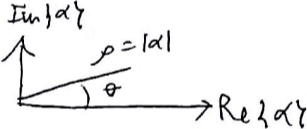
\includegraphics[width=0.3\textwidth]{./images/4-coherent-rep}
	\caption{Projection of a coherent state $\ket{\alpha}$ over the real and imaginary lines}
	\label{fig:coherent-rep}
\end{figure}

\subsubsection*{Coherent states are minimal states}
\begin{thm}[Heisenberg principle]
	If $\comm*{\hat{A}}{\hat{B}} = \hat{C}$, therefore $\Delta \hat{A} \cdot \Delta \hat{B} \geq \dfrac{1}{2}\ev*{\hat{C}}$.
\end{thm}

\begin{defi}[Quadratures of the electromagnetic field]
	The quadratures are hermitian operators that represent the real and imaginary parts of the complex amplitude represented by $\hat{a}$:
	\begin{align}
		\hat{X}_{1} = \hat{a}\sdag + \hat{a} \qc \hat{X}_{2} = i \qty(\hat{a}\sdag - \hat{a})
	\end{align}
	Therefore,
	\begin{align*}
		\underset{1\text{ mode}}{\trn{\va{E}}} = \mc{E}_{\omega} \vu{\epsilon} \qty{ \hat{X}_{1} \sin(\omega t - \va{k}\vdot\va{r}) - \hat{X}_{2} \cos(\omega t - \va{k}\vdot\va{r}) }
	\end{align*}
	The commutation relation between the two quadratures is
	\begin{align}
		\comm{\hat{X}_{1}}{\hat{X}_{2}} = 2i
	\end{align}
\end{defi}

\begin{itemize}
	\item The expected values of the quadratures are $\ev*{\hat{X}_{1}} = 2 \Re{\alpha}$, $\ev*{\hat{X}_{2}} = 2 \Im{\alpha}$.
	\item The uncertainties of the quadratures are $\Delta \hat{X}_{1,2} \equiv 1$. This is called the standard quantum limit.
\end{itemize}

Therefore, coherent states, $\ket{\alpha}$, are minimal states, meaning that they saturate the Heisenberg principle:
\begin{align}
	\Delta \hat{X}_{1} \Delta \hat{X}_{2} \equiv 1
\end{align}

\subsubsection*{Coherent states can be considered displaced vacuum}
\begin{thm}[Baker--Campbell--Hausdorff formula]
	If $\comm*{\hat{A}}{\comm*{\hat{A}}{\hat{B}}} = \comm*{\hat{B}}{\comm*{\hat{A}}{\hat{B}}} = 0$, therefore
	\begin{align}\label{eq:dumbledore}
		e^{\hat{A}+\hat{B}} = e^{\hat{A}} e^{\hat{B}} e^{-\comm*{\hat{A}}{\hat{B}}/2}
	\end{align}
\end{thm}
\begin{defi}[Displacement operator]
	The displacement operator is a unitary operator:
	\begin{align}
		\hat{\mc{D}}(\alpha) = \exp{\alpha \hat{a}\sdag + \alpha\sast \hat{a}}
	\end{align}
\end{defi}
\begin{subequations}
The displacement operator is not hermitian: $\hat{\mc{D}}\sdag(\alpha) \equiv \hat{\mc{D}}(-\alpha) = \hat{\mc{D}}^{-1}(\alpha)$. It can be shown that
\begin{align}
	\hat{\mc{D}}\sdag(\alpha) \hat{a} \hat{\mc{D}}(\alpha) &= \hat{a} + \alpha \\
	\hat{\mc{D}}\sdag(\alpha) \hat{a}\sdag \hat{\mc{D}}(\alpha) &= \hat{a}\sdag + \alpha\sast
\end{align}
\end{subequations}

Therefore, coherent states can be interpreted as displaced vacuum:
\begin{align}
	\ket{a} = \hat{\mc{D}}(\alpha) \ket{0}
\end{align}
Using the Baker--Campbell--Hausdorff formula \eqref{eq:dumbledore}, we can get $\ket{\alpha}$ in the Fock states basis.

\begin{itemize}
	\item Fock states are not minimal: $\braket{\hat{X}_{1,2}}{n} = 0$, $(\Delta \hat{X}_{1,2})^{2}_{\ket{n}} = 2n + 1$.
	\item But vacuum is: $(\Delta \hat{X}_{1,2})_{\ket{0}} \equiv 1$.
\end{itemize}

\begin{figure}[H]
	\centering
	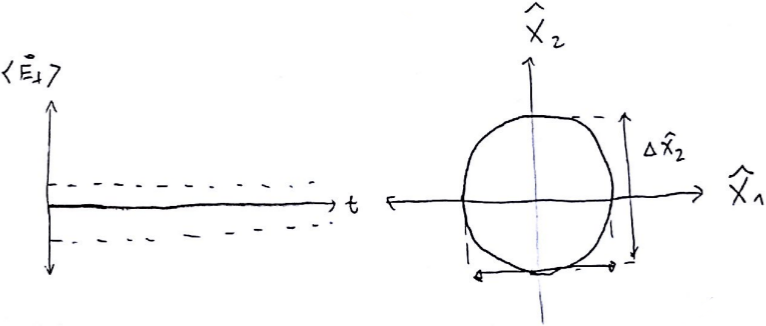
\includegraphics[width=0.7\textwidth]{./images/4-vacuum}
	% \caption{Representation of a the vacuum in the phase space}
	\caption{Representation of a the vacuum}
	\label{fig:vacuum}
\end{figure}
\begin{figure}[H]
	\centering
	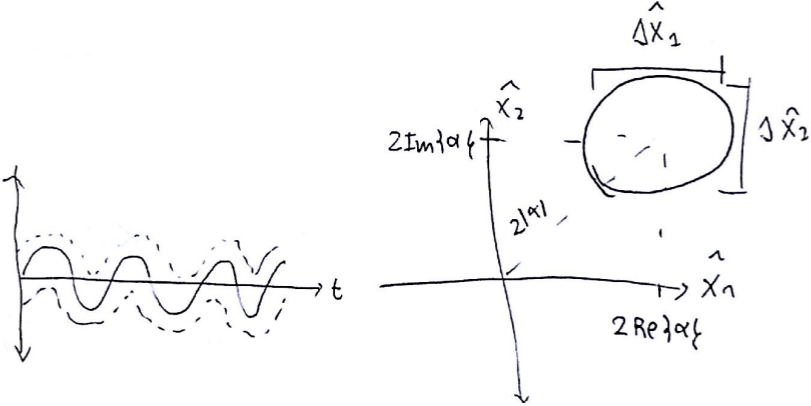
\includegraphics[width=0.75\textwidth]{./images/4-coherent}
	% \caption{Representation of a coherent state as displaced vacuum in the phase space}
	\caption{Representation of a coherent state as displaced vacuum}
	\label{fig:coherent}
\end{figure}

%-----------------------------------------------------------------
\subsection{Squeezed states}
\begin{defi}[Squeezed state, $\ket{s}$]
	A squeezed state is minimal ($\Delta \hat{X}_{1} \Delta \hat{X}_{2} \equiv 1$). Nonetheless, squeezed states break the standard quantum limit:
	\begin{align*}
		\begin{cases}
			\Delta \hat{X}_{1} < 1 \Leftrightarrow \Delta \hat{X}_{2} > 1 \\
			\Delta \hat{X}_{2} < 1 \Leftrightarrow \Delta \hat{X}_{1} > 1
		\end{cases}
	\end{align*}
\end{defi}
\begin{figure}[H]
	\centering
	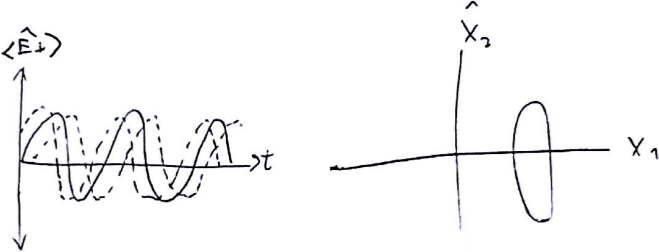
\includegraphics[width=0.7\textwidth]{./images/4-squeezed-x1}
	\caption{Representation of a squeezed state with $\Delta \hat{X}_{1} < 1$}
	\label{fig:squeezed1}
\end{figure}

\begin{figure}[H]
	\centering
	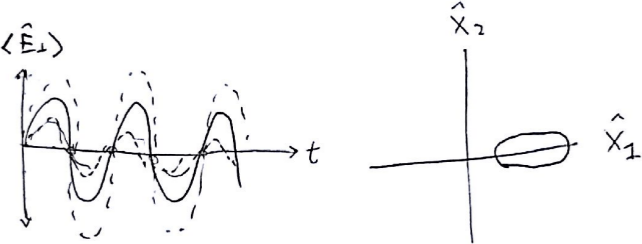
\includegraphics[width=0.7\textwidth]{./images/4-squeezed-x2}
	\caption{Representation of a squeezed state with $\Delta \hat{X}_{2} < 1$}
	\label{fig:squeezed2}
\end{figure}
\subsubsection*{Squeezing operator}
\begin{defi}[Squeezing operator]
	The squeezing operator is a unitary operator:
	\begin{align}
		\hat{\mc{S}}(z) = \exp{\frac{1}{2} \qty[z\sast \hat{a}^{2} - z \hat{a}\sdag^{2}]}
	\end{align}
	where $z = r e^{i \phi}$, $r$ being the squeezing parameter.
\end{defi}

\begin{subequations}
The squeezing operator is not hermitian: $\hat{\mc{S}}\sdag(z) \equiv \hat{\mc{S}}(-z) = \hat{\mc{S}}^{-1}(z)$. It can be shown that
\begin{align}
	\hat{\mc{S}}\sdag(z) \hat{a} \hat{\mc{S}}(z) &= \hat{a} \cosh r - \hat{a}\sdag e^{i\phi} \sinh r \\
	\hat{\mc{S}}\sdag(z) \hat{a}\sdag \hat{\mc{S}}(z) &= \hat{a}\sdag \cosh r - \hat{a} e^{-i\phi} \sinh r
\end{align}
\end{subequations}
Since squeezed states break the standard quantum limit, they can be interpreted as squeezed coherent states:
\begin{align}
	\ket{s} = \hat{\mc{S}}(z) \ket{\alpha}
\end{align}
For $\phi = 0$, $(\Delta \hat{X}_{1})^{2}_{\ket{s}} = e^{-2r} (\Delta \hat{X}_{1})^{2}_{\ket{\alpha}}$, and $(\Delta \hat{X}_{2})^{2}_{\ket{s}} = e^{2r} (\Delta \hat{X}_{2})^{2}_{\ket{\alpha}}$.
